\documentclass[12pt]{ociamthesis}  % default square logo 
%\documentclass[12pt,beltcrest]{ociamthesis} % use old belt crest logo
%\documentclass[12pt,shieldcrest]{ociamthesis} % use older shield crest logo

%load any additional packages
\usepackage{amssymb}
\usepackage{listings}

\usepackage{color}
 
\definecolor{codegreen}{rgb}{0,0.6,0}
\definecolor{codegray}{rgb}{0.5,0.5,0.5}
\definecolor{codepurple}{rgb}{0.58,0,0.82}
\definecolor{backcolour}{rgb}{0.95,0.95,0.92}
 
\lstdefinestyle{mystyle}{
    backgroundcolor=\color{backcolour},   
    commentstyle=\color{codegreen},
    keywordstyle=\color{magenta},
    numberstyle=\tiny\color{codegray},
    stringstyle=\color{codepurple},
    basicstyle=\footnotesize,
    breakatwhitespace=false,         
    breaklines=true,                 
    captionpos=b,                    
    keepspaces=true,                 
    numbers=left,                    
    numbersep=5pt,                  
    showspaces=false,                
    showstringspaces=false,
    showtabs=false,                  
    tabsize=2,
    language=python
}
 
\lstset{style=mystyle}
%input macros (i.e. write your own macros file called mymacros.tex 
%and uncomment the next line)
%\include{mymacros}

\title{Modul Praktikum \\[1ex]     %your thesis title,
        Kecerdasan Buatan}   %note \\[1ex] is a line break in the title

\author{Rolly Maulana Awangga}             %your name
\college{0410118609\\[5ex]
Applied Bachelor of Informatics Engineering}  %your college

%\renewcommand{\submittedtext}{change the default text here if needed}
\degree{Politeknik Pos Indonesia}     %the degree
\degreedate{Bandung 2019}         %the degree date

%end the preamble and start the document
\begin{document}

%this baselineskip gives sufficient line spacing for an examiner to easily
%markup the thesis with comments
\baselineskip=18pt plus1pt

%set the number of sectioning levels that get number and appear in the contents
\setcounter{secnumdepth}{3}
\setcounter{tocdepth}{3}


\maketitle                  % create a title page from the preamble info
\begin{dedication}
`Jika Kamu tidak dapat menahan lelahnya belajar, \\
Maka kamu harus sanggup menahan perihnya Kebodohan.'\\ 
~Imam Syafi'i~\\
\end{dedication}        % include a dedication.tex file
\begin{acknowledgements}
Pertama-tama kami panjatkan puji dan syukur kepada Allah SWT yang telah memberikan rahmat dan hidayah-Nya sehingga Buku Pedoman Tingkat Akhir ini dapat diselesaikan.
\end{acknowledgements}   % include an acknowledgements.tex file
\begin{abstract}
	Buku Pedoman ini dibuat dengan tujuan memberikan acuan, bagi mahasiswa Tingkat Akhir dan dosen
	Pembimbing. Pada intinya buku ini menjelaskan secara lengkap tentang Standar pengerjaan Intership  dan 
	Tugas Akhir
	di Program Studi D4 Teknik Informatika, dan juga mengatur mekanisme, teknik penulisan, serta
	penilaiannya.Dengan demikian diharapkan semua pihak yang terlibat dalam aktivitas Bimbingan Mahasiswa Tingkat Akhir
	berjalan lancar dan sesuai dengan standar.
\end{abstract}          % include the abstract

\begin{romanpages}          % start roman page numbering
\tableofcontents            % generate and include a table of contents
\listoffigures              % generate and include a list of figures
\end{romanpages}            % end roman page numbering

%now include the files of latex for each of the chapters etc
\chapter{Mengenal Kecerdasan Buatan dan Scikit-Learn}
Buku umum yang digunakan adalah \cite{russell2016artificial} dan  
untuk sebelum UTS menggunakan buku \textit{Python Artificial Intelligence Projects for Beginners}\cite{eckroth2018python}.
Dengan praktek menggunakan python 3 dan editor anaconda dan library python scikit-learn.
Tujuan pembelajaran pada pertemuan pertama antara lain:
\begin{enumerate}
\item
Mengerti definisi kecerdasan buatan, sejarah kecerdasan buatan, perkembangan dan penggunaan di perusahaan
\item
Memahami cara instalasi dan pemakaian sci-kit learn
\item
Memahami cara penggunaan variabel explorer di spyder
\end{enumerate}
Tugas dengan cara dikumpulkan dengan pull request ke github dengan menggunakan latex pada repo yang dibuat oleh asisten riset.

\section{Teori}
Praktek teori penunjang yang dikerjakan :
\begin{enumerate}
\item
Buat Resume Definisi, Sejarah dan perkembangan Kecerdasan Buatan, dengan bahasa yang mudah dipahami dan dimengerti. Buatan sendiri bebas plagiat(10)
\item
Buat Resume mengenai definisi supervised learning, klasifikasi, regresi dan unsupervised learning. Data set, training set dan testing set.(10)
\end{enumerate}

\section{Instalasi}
Membuka https://scikit-learn.org/stable/tutorial/basic/tutorial.html. Dengan menggunakan bahasa yang mudah dimengerti dan bebas plagiat. 
Dan wajib skrinsut dari komputer sendiri.
\begin{enumerate}
\item
Instalasi spyder, mencoba kompilasi dan uji coba variabel explorer(10)
\item
Mencoba Loading an example dataset, menjelaskan maksud dari tulisan tersebut dan mengartikan per baris(10)
\item
Mencoba Learning and predicting, menjelaskan maksud dari tulisan tersebut dan mengartikan per baris(10)
\item
mencoba Model persistence, menjelaskan maksud dari tulisan tersebut dan mengartikan per baris(10)
\item 
Mencoba Conventions, menjelaskan maksud dari tulisan tersebut dan mengartikan per baris(10)
\end{enumerate}


\section{Penanganan Error}
Dari percobaan yang dilakukan di atas, apabila mendapatkan error maka:

\begin{enumerate}
	\item
	skrinsut error(10)
	\item
Tuliskan kode eror dan jenis errornya (10)
	\item
Solusi pemecahan masalah error tersebut(10)

\end{enumerate}


\chapter{Related Works}

Your related works, and your purpose and contribution which must be different as below.

\section{Same Topics}
Cite every latest journal with same topic
\subsection{Topic 1}
cite for first topic

\subsection{Topic 2}
if you have two topics you can include here to


\section{Same Method}
write and cite latest journal with same method

\subsection{Method 1}
cite and paraphrase method 1

\subsection{Method 2}
cite and paraphrase method 2 if you have more method please add new subsection.

 
\chapter{Prediksi dengan Random Forest}

Untuk pratikum saati ini menggunakan buku \textit{Python Artificial Intelligence Projects for Beginners}\cite{eckroth2018python}. Dengan praktek menggunakan python 3 dan editor anaconda dan library python scikit-learn.
Dataset ada di https://github.com/PacktPublishing/Python-Artificial-Intelligence-Projects-for-Beginners .
Tujuan pembelajaran pada pertemuan pertama antara lain:
\begin{enumerate}
\item
Mengerti implementasi klasifikasi dan teknik evaluasi
\item
Memprediksi spesies burung dengan random forest
\item
Memahami Confusion Matrix.
\end{enumerate}
Tugas dengan cara dikumpulkan dengan pull request ke github dengan menggunakan latex pada repo yang dibuat oleh asisten riset. Kode program menggunakan input listing ditaruh di folder src ekstensi .py dan dipanggil ke latex dengan input listings. Tulisan dan kode tidak boleh plagiat, menggunakan bahasa indonesia yang sesuai dengan gaya bahasa buku teks.

\section{Teori}
Random Forest adalah hasil voting dari beberapa decission tree yang masing-masing memegang atribut yang berbeda. Jadi setiap decission tree spesifik terhadap atribut tersebut yang merupakan bagian kecil dari keseluruhan atribut di data set. Hindari RF jika atribut terlalu sedikit untuk membentuk beberapa tree. Pada praktek kali ini mengggunakan dataset spesies burung yang diambil dari situs (http://www.vision.caltech.edu/visipedia/CUB-200-2011.html). Didalmnya terdapat 12.000 foto dari 200 spesies yang berbeda. Yang akan kita pakai untuk RF hanya atribut dari burunynya saja seperti ukuran, bentuk dan warna. Data tersebut diberi label secara manual oleh manusia dengan memanfaatkan jasa dari Amazon's Mechanical Turk.

\subsection{Random Forest}
Pertama dataset kita baca terlebih dahulu.
\begin{lstlisting}[caption=Fungsi Sederhana,label={lst:fungsisederhana}]
import pandas as pd

# some lines have too many fields (?), so skip bad lines
imgatt = pd.read_csv("data/CUB_200_2011/attributes/image_attribute_labels.txt",
                     sep='\s+', header=None, error_bad_lines=False, warn_bad_lines=False,
                     usecols=[0,1,2], names=['imgid', 'attid', 'present'])

\end{lstlisting}

Melihat sebagian data awal, dengan menggunakan listing \ref{lst:3.1}.

\begin{lstlisting}[caption=Melihat sebagian data awal,label={lst:3.1}]
imgatt.head()
\end{lstlisting}

Melihat jumlah data menggunakan listing \ref{lst:3.2}.
\begin{lstlisting}[caption=Mengetahui jumlah data,label={lst:3.2}]
imgatt.shape
\end{lstlisting}

Merubah atribut menjadi kolom dengan menggunakan pivot layaknya excel. lalu kita cek isinya dengan menggunakan perintah pada listing \ref{lst:3.3}.
\begin{lstlisting}[caption=Pivot dataset,label={lst:3.3}]
imgatt2 = imgatt.pivot(index='imgid', columns='attid', values='present')

imgatt2.head()
imgatt2.shape
\end{lstlisting}


Sekarang kita akan meload jawabannya yang berisi apakah burung itu termasuk dalam spesies yang mana. Dua kolomnya adalah imgid dan label. Dan melakukan pivot yang mana imgid menjadi index yang artinya unik perintahnya ada di listing \ref{lst:3.6}. Lalu kita cek kembali datanya. 
\begin{lstlisting}[caption=Fungsi Sederhana,label={lst:3.6}]
imglabels = pd.read_csv("data/CUB_200_2011/image_class_labels.txt", 
                        sep=' ', header=None, names=['imgid', 'label'])

imglabels = imglabels.set_index('imgid')


imglabels.head()
imglabels.shape
\end{lstlisting}

Karena isinya sama kita bisa melakukan join antara dua data. Sehingga kita akan mendapatkan data ciri dan data jawabannya atau labelnya sehingga bisa dikatekorikan supervised learning. maka perintah untuk menggabungkan kedua data dan kemudian kita melakukan pemisahan antara data set untuk training dan test dengan perintah di listing \ref{lst:3.7}.
\begin{lstlisting}[caption=Fungsi Sederhana,label={lst:3.7}]
df = imgatt2.join(imglabels)
df = df.sample(frac=1)
\end{lstlisting}

Kemudian drop label yang didepan, dan gunakan label yang paling belakang yang baru di join dengan perintah listing \ref{lst:3.8}.
\begin{lstlisting}[caption=Fungsi Sederhana,label={lst:3.8}]
df_att = df.iloc[:, :312]
df_label = df.iloc[:, 312:]
\end{lstlisting}
Kita bisa mengecek isinya dengan perintah listing \ref{lst:3.9}.
\begin{lstlisting}[caption=Fungsi Sederhana,label={lst:3.9}]
df_att.head()
df_label.head()
\end{lstlisting}

Kita bagi menjadi dua bagian, 8000 row pertama sebagai data training sisanya sebagai data testing dengan perintah listing \ref{lst:3.10}.
\begin{lstlisting}[caption=Fungsi Sederhana,label={lst:3.10}]
df_train_att = df_att[:8000]
df_train_label = df_label[:8000]
df_test_att = df_att[8000:]
df_test_label = df_label[8000:]

df_train_label = df_train_label['label']
df_test_label = df_test_label['label']
\end{lstlisting}

Kita panggil kelas RandomForestClassifier. max features diartikan sebagai berapa banyak kolom pada setiap tree dengan perintah listing \ref{lst:3.11}.
\begin{lstlisting}[caption=Fungsi Sederhana,label={lst:3.11}]
from sklearn.ensemble import RandomForestClassifier
clf = RandomForestClassifier(max_features=50, random_state=0, n_estimators=100)

\end{lstlisting}
Kemudian lakukan fit untuk membangun random forest yang sudah ditentukan dengan maksimum fitur sebanya 50 untuk perpohonnya dengan perintah listing \ref{lst:3.12}.

\begin{lstlisting}[caption=Fungsi Sederhana,label={lst:3.12}]
clf.fit(df_train_att, df_train_label)
\end{lstlisting}
Hasilnya bisa kita dapatkan dengan perintah predict dengan perintah listing \ref{lst:3.13}.
\begin{lstlisting}[caption=Fungsi Sederhana,label={lst:3.13}]
print(clf.predict(df_train_att.head()))
\end{lstlisting}

Untuk besaran akurasinya dengan perintah listing \ref{lst:3.14}
\begin{lstlisting}[caption=Fungsi Sederhana,label={lst:3.14}]
clf.score(df_test_att, df_test_label)
\end{lstlisting}

\subsection{Confusion Matrix}
Dari RF kita coba petakan ke dalam Confusion Matrix dan lihat hasilnya dengan perintah listing \ref{lst:3.15}.
\begin{lstlisting}[caption=Fungsi Sederhana,label={lst:3.15}]
from sklearn.metrics import confusion_matrix
pred_labels = clf.predict(df_test_att)
cm = confusion_matrix(df_test_label, pred_labels)

cm
\end{lstlisting}

Kemudian kita plot dengan perintah
\begin{lstlisting}[caption=Fungsi Sederhana,label={lst:3.16}]
import matplotlib.pyplot as plt
import itertools
def plot_confusion_matrix(cm, classes,
                          normalize=False,
                          title='Confusion matrix',
                          cmap=plt.cm.Blues):
    """
    This function prints and plots the confusion matrix.
    Normalization can be applied by setting `normalize=True`.
    """
    if normalize:
        cm = cm.astype('float') / cm.sum(axis=1)[:, np.newaxis]
        print("Normalized confusion matrix")
    else:
        print('Confusion matrix, without normalization')

    print(cm)

    plt.imshow(cm, interpolation='nearest', cmap=cmap)
    plt.title(title)
    #plt.colorbar()
    tick_marks = np.arange(len(classes))
    plt.xticks(tick_marks, classes, rotation=90)
    plt.yticks(tick_marks, classes)

    fmt = '.2f' if normalize else 'd'
    thresh = cm.max() / 2.
    #for i, j in itertools.product(range(cm.shape[0]), range(cm.shape[1])):
    #    plt.text(j, i, format(cm[i, j], fmt),
    #             horizontalalignment="center",
    #             color="white" if cm[i, j] > thresh else "black")

    plt.tight_layout()
    plt.ylabel('True label')
    plt.xlabel('Predicted label')

\end{lstlisting}

 Agar plot sumbunya sesuai dengan nama datanya maka kita set dengan perintah
\begin{lstlisting}[caption=Fungsi Sederhana,label={lst:3.17}]
birds = pd.read_csv("data/CUB_200_2011/classes.txt",
                    sep='\s+', header=None, usecols=[1], names=['birdname'])
birds = birds['birdname']
birds

\end{lstlisting}

Lalu kita plot
\begin{lstlisting}[caption=Fungsi Sederhana,label={lst:3.18}]
import numpy as np
np.set_printoptions(precision=2)
plt.figure(figsize=(60,60), dpi=300)
plot_confusion_matrix(cm, classes=birds, normalize=True)
plt.show()
\end{lstlisting}



\subsection{Mencoba dengan metode Decission Tree dan SVM}
Kita coba menggunakan Decission tree 
\begin{lstlisting}[caption=Fungsi Sederhana,label={lst:3.19}]
from sklearn import tree
clftree = tree.DecisionTreeClassifier()
clftree.fit(df_train_att, df_train_label)
clftree.score(df_test_att, df_test_label)
\end{lstlisting}
Kita coba menggunakan SVM
\begin{lstlisting}[caption=Fungsi Sederhana,label={lst:3.20}]
from sklearn import svm
clfsvm = svm.SVC()
clfsvm.fit(df_train_att, df_train_label)
clfsvm.score(df_test_att, df_test_label)
\end{lstlisting}

\subsection{Pengecekan Cross Validation}
Pengeceken Cross Validation untuk random forest
\begin{lstlisting}[caption=Fungsi Sederhana,label={lst:3.21}]
from sklearn.model_selection import cross_val_score
scores = cross_val_score(clf, df_train_att, df_train_label, cv=5)
# show average score and +/- two standard deviations away (covering 95% of scores)
print("Accuracy: %0.2f (+/- %0.2f)" % (scores.mean(), scores.std() * 2))
\end{lstlisting}
untuk decission tree
\begin{lstlisting}[caption=Fungsi Sederhana,label={lst:3.22}]
scorestree = cross_val_score(clftree, df_train_att, df_train_label, cv=5)
print("Accuracy: %0.2f (+/- %0.2f)" % (scorestree.mean(), scorestree.std() * 2))
\end{lstlisting}
untuk SVM
\begin{lstlisting}[caption=Fungsi Sederhana,label={lst:3.23}]
scoressvm = cross_val_score(clfsvm, df_train_att, df_train_label, cv=5)
print("Accuracy: %0.2f (+/- %0.2f)" % (scoressvm.mean(), scoressvm.std() * 2))
\end{lstlisting}



\subsection{Mengatahui komponen komponen informasi}
Untuk mengetahui berapa banyak tree yang dibuat, berapa banyak atribut yang dipakai dan informasi lainnya menggunakan kode
\begin{lstlisting}[caption=Fungsi Sederhana,label={lst:3.24}]
max_features_opts = range(5, 50, 5)
n_estimators_opts = range(10, 200, 20)
rf_params = np.empty((len(max_features_opts)*len(n_estimators_opts),4), float)
i = 0
for max_features in max_features_opts:
    for n_estimators in n_estimators_opts:
        clf = RandomForestClassifier(max_features=max_features, n_estimators=n_estimators)
        scores = cross_val_score(clf, df_train_att, df_train_label, cv=5)
        rf_params[i,0] = max_features
        rf_params[i,1] = n_estimators
        rf_params[i,2] = scores.mean()
        rf_params[i,3] = scores.std() * 2
        i += 1
        print("Max features: %d, num estimators: %d, accuracy: %0.2f (+/- %0.2f)" %               (max_features, n_estimators, scores.mean(), scores.std() * 2))

\end{lstlisting}
Dan kita bisa melakukan plot informasi ini dengan kode
\begin{lstlisting}[caption=Fungsi Sederhana,label={lst:3.25}]
import matplotlib.pyplot as plt
from mpl_toolkits.mplot3d import Axes3D
from matplotlib import cm
fig = plt.figure()
fig.clf()
ax = fig.gca(projection='3d')
x = rf_params[:,0]
y = rf_params[:,1]
z = rf_params[:,2]
ax.scatter(x, y, z)
ax.set_zlim(0.2, 0.5)
ax.set_xlabel('Max features')
ax.set_ylabel('Num estimators')
ax.set_zlabel('Avg accuracy')
plt.show()
\end{lstlisting}




\section{Soal Teori}
Praktek teori penunjang yang dikerjakan(nilai 5 per nomor, untuk hari pertama) :
\begin{enumerate}
\item
Jelaskan apa itu random forest, sertakan gambar ilustrasi buatan sendiri.
\item
Jelaskan cara membaca dataset dan artikan makna setiap file dan isi filenya.
\item
Jelaskan apa itu evaluasi dan akurasi dari buku dan disertai ilustrasi contoh dengan gambar sendiri
\item
Jelaskan bagaimana cara membuat dan membaca confusion matrix, buat confusion matrix buatan sendiri.
\item
Jelaskan bagaimana K-fold cross validation bekerja dengan gambar ilustrasi contoh buatan sendiri.
\item
Jelaskan apa itu decision tree dengan gambar ilustrasi contoh buatan sendiri.
\item
Jelaskan apa itu information gain dan entropi dengan gambar ilustrasi buatan sendiri.
\end{enumerate}

\section{scikit-learn}
Dataset ambil di https://github.com/PacktPublishing/Python-Artificial-Intelligence-Projects-for-Beginners folder Chapter01.
Tugas anda adalah, dataset ganti menggunakan \textbf{student-mat.csv} dan mengganti semua nama variabel dari kode di bawah ini dengan nama-nama makanan (NPM mod 3=0), kota (NPM mod 3=1), buah (NPM mod 3=2), . Jalankan satu per satu kode tersebut di spyder dengan menggunakan textit{Run current cell}. Kemudian Jelaskan dengan menggunakan bahasa yang mudah dimengerti dan bebas plagiat dan wajib skrinsut dari komputer sendiri masing masing nomor di bawah ini(nilai 5 masing masing pada hari kedua).

\begin{enumerate}

\item
\begin{verbatim}
	# load dataset (student mat pakenya)
	import pandas as pd
	d = pd.read_csv('student-mat.csv', sep=';')
	len(d)
\end{verbatim}
\item
\begin{verbatim}
	# generate binary label (pass/fail) based on G1+G2+G3 
	# (test grades, each 0-20 pts); threshold for passing is sum>=30
	d['pass'] = d.apply(lambda row: 1 if (row['G1']+row['G2']+row['G3']) 
											>= 35 else 0, axis=1)
	d = d.drop(['G1', 'G2', 'G3'], axis=1)
	d.head()
\end{verbatim}
\item
\begin{verbatim}
	# use one-hot encoding on categorical columns
	d = pd.get_dummies(d, columns=['sex', 'school', 'address', 
									'famsize', 
									'Pstatus', 'Mjob', 'Fjob', 
	                               'reason', 'guardian', 'schoolsup', 
								   'famsup', 'paid', 'activities',
	                               'nursery', 'higher', 'internet', 
									'romantic'])
	d.head()
\end{verbatim}
\item
\begin{verbatim}
	# shuffle rows
	d = d.sample(frac=1)
	# split training and testing data
	d_train = d[:500]
	d_test = d[500:]

	d_train_att = d_train.drop(['pass'], axis=1)
	d_train_pass = d_train['pass']

	d_test_att = d_test.drop(['pass'], axis=1)
	d_test_pass = d_test['pass']

	d_att = d.drop(['pass'], axis=1)
	d_pass = d['pass']

	# number of passing students in whole dataset:
	import numpy as np
	print("Passing: %d out of %d (%.2f%%)" % (np.sum(d_pass), len(d_pass), 
	       100*float(np.sum(d_pass)) / len(d_pass)))
\end{verbatim}
\item 
\begin{verbatim}
	# fit a decision tree
	from sklearn import tree
	t = tree.DecisionTreeClassifier(criterion="entropy", max_depth=5)
	t = t.fit(d_train_att, d_train_pass)
\end{verbatim}
\item
\begin{verbatim}
	# visualize tree
	import graphviz
	dot_data = tree.export_graphviz(t, out_file=None, label="all", 
									impurity=False, proportion=True,
	                                feature_names=list(d_train_att), 
									class_names=["fail", "pass"], 
	                                filled=True, rounded=True)
	graph = graphviz.Source(dot_data)
	graph
\end{verbatim}
\item
\begin{verbatim}
	# save tree
	tree.export_graphviz(t, out_file="student-performance.dot", 
						 label="all", impurity=False, 
						 proportion=True,
	                     feature_names=list(d_train_att), 
	                     class_names=["fail", "pass"], 
	                     filled=True, rounded=True)
\end{verbatim}
\item
\begin{verbatim}
	t.score(d_test_att, d_test_pass)
\end{verbatim}
\item
\begin{verbatim}
	from sklearn.model_selection import cross_val_score
	scores = cross_val_score(t, d_att, d_pass, cv=5)
	# show average score and +/- two standard deviations away 
	#(covering 95% of scores)
	print("Accuracy: %0.2f (+/- %0.2f)" % (scores.mean(), scores.std() * 2))
\end{verbatim}
\item 
\begin{verbatim}
	for max_depth in range(1, 20):
	    t = tree.DecisionTreeClassifier(criterion="entropy", 
			max_depth=max_depth)
	    scores = cross_val_score(t, d_att, d_pass, cv=5)
	    print("Max depth: %d, Accuracy: %0.2f (+/- %0.2f)" % 
				(max_depth, scores.mean(), scores.std() * 2)
			 )
\end{verbatim}
\item
\begin{verbatim}
	depth_acc = np.empty((19,3), float)
	i = 0
	for max_depth in range(1, 20):
	    t = tree.DecisionTreeClassifier(criterion="entropy", 
			max_depth=max_depth)
	    scores = cross_val_score(t, d_att, d_pass, cv=5)
	    depth_acc[i,0] = max_depth
	    depth_acc[i,1] = scores.mean()
	    depth_acc[i,2] = scores.std() * 2
	    i += 1

	depth_acc
\end{verbatim}
\item 
\begin{verbatim}
	import matplotlib.pyplot as plt
	fig, ax = plt.subplots()
	ax.errorbar(depth_acc[:,0], depth_acc[:,1], yerr=depth_acc[:,2])
	plt.show()
\end{verbatim}

\end{enumerate}


\section{Penanganan Error}
Dari percobaan yang dilakukan di atas, error yang kita dapatkan di dokumentasikan dan di selesaikan(nilai 5 hari kedua):

\begin{enumerate}
	\item
skrinsut error
	\item
Tuliskan kode eror dan jenis errornya
	\item
Solusi pemecahan masalah error tersebut

\end{enumerate}


\chapter{Klasifikasi Teks}

Untuk pratikum saati ini menggunakan buku \textit{Python Artificial Intelligence Projects for Beginners}\cite{eckroth2018python}. Dengan praktek menggunakan python 3 dan editor anaconda dan library python scikit-learn.
Kode program ada di https://github.com/PacktPublishing/Python-Artificial-Intelligence-Projects-for-Beginners .
Tujuan pembelajaran pada pertemuan pertama antara lain:
\begin{enumerate}
\item
Mengerti implementasi klasifikasi pada teks
\item
Mengerti teknik machine learning
\item
Memahami Bag of Words
\end{enumerate}

Tugas dengan cara dikumpulkan dengan pull request ke github dengan menggunakan latex pada repo yang dibuat oleh asisten riset. Kode program menggunakan input listing ditaruh di folder src ekstensi .py dan dipanggil ke latex dengan input listings. Tulisan dan kode tidak boleh plagiat, menggunakan bahasa indonesia yang sesuai dengan gaya bahasa buku teks.

\section{Teori}
Menggunakan teknik bag-of-words pada klasifikasi berbasis text dan kata untuk mengklasifikasikan komentar yang ada di internet sebagai spam atau bukan. Atau bisa juga untuk melakukan identifikasi sebuah review apakah positive atau negatif.


\subsection{Vektorisasi data}
Pertama kita lakukan vektorisasi dari dataset. Lankah pertama kita baca terlebih dahulu dengan perintah \ref{lst:4.0}.
\begin{lstlisting}[caption=Membaca data file txt,label={lst:4.0}]
import pandas as pd
d = pd.read_csv("Youtube01-Psy.csv")
\end{lstlisting}

Memanggil library vektorisasi dari sci-kit lern, dengan menggunakan listing \ref{lst:4.1}.

\begin{lstlisting}[caption=Instansiasi Vektorizer,label={lst:4.1}]
from sklearn.feature_extraction.text import CountVectorizer
vectorizer = CountVectorizer()
\end{lstlisting}

Memilih kolom CONTENT dari dataframe d untuk di vektorisasi kemudian menampungnya pada variabel dvec menggunakan listing \ref{lst:4.2}.
\begin{lstlisting}[caption=Vektorisasi data dari atribut CONTENT,label={lst:4.2}]
dvec = vectorizer.fit_transform(d['CONTENT'])
dvec
\end{lstlisting}

Melihat daftar kata yang di vektorisasi. lalu kita simpan isinya pada variabel daptarkata dengan menggunakan perintah pada listing \ref{lst:4.3}.
\begin{lstlisting}[caption=Mendapatkan Daftar Kata,label={lst:4.3}]
daptarkata=vectorizer.get_feature_names()
\end{lstlisting}


Lakukan pengocokan data sehingga data terlihat random, perintahnya ada di listing \ref{lst:4.6}. Lalu kita cek kembali datanya pada variabel dshuf. 
\begin{lstlisting}[caption=Mengocok Data Frame,label={lst:4.6}]
dshuf = d.sample(frac=1)
\end{lstlisting}

kemudian kita melakukan pemisahan antara data set untuk training dan test dengan perintah di listing \ref{lst:4.7}.
\begin{lstlisting}[caption=Memisahkan data frame,label={lst:4.7}]
d_train=dshuf[:300]
d_test=dshuf[300:]
\end{lstlisting}

Kita lakukan training perintah listing \ref{lst:4.8}.
\begin{lstlisting}[caption=Training pada vektorisasi atau yang disebut transform dan fit,label={lst:4.8}]
d_train_att=vectorizer.fit_transform(d_train['CONTENT'])
d_train_att
\end{lstlisting}

Lalu kita lakukan transformasi saja tanpa training pada data testing dengan perintah listing \ref{lst:4.9}.
\begin{lstlisting}[caption=Transform tanpa fit dari data testing,label={lst:4.9}]
d_test_att=vectorizer.transform(d_test['CONTENT'])
d_test_att
\end{lstlisting}

Pengambilan label klasifikasi spam dari kolom CLASS dengan perintah listing \ref{lst:4.10}.
\begin{lstlisting}[caption=Pengambilan label dari data testing dan training,label={lst:4.10}]
d_train_label=d_train['CLASS']
d_test_label=d_test['CLASS']
\end{lstlisting}



\subsection{Klasifikasi dengan Random Forest}
Setelah lakukan vektorisasi. Kita panggil kelas RandomForestClassifier. dengan n estimators sebanyak 80 yang artinya kita akan membuat 80 tree dengan tanpa batasan pengambilan atribut atau kolom dengan perintah listing \ref{lst:4.11}.
\begin{lstlisting}[caption=Instansiasi kelas Random Forest,label={lst:4.11}]
from sklearn.ensemble import RandomForestClassifier
clf=RandomForestClassifier(n_estimators=80)
\end{lstlisting}


Kemudian lakukan fit untuk membangun random forest yang sudah ditentukan dengan banyak tree sebanyak 80 dengan perintah listing \ref{lst:4.12}.
\begin{lstlisting}[caption=Fitting random forest dengan dataset training,label={lst:4.12}]
clf.fit(d_train_att,d_train_label)
\end{lstlisting}


Hasilnya bisa kita lakukan prediksi dari data testing dengan perintah listing \ref{lst:4.13}.
\begin{lstlisting}[caption=Melihat Hasil prediksi,label={lst:4.13}]
clf.predict(d_test_att)
\end{lstlisting}

Untuk besaran skornya dengan perintah listing \ref{lst:4.14}
\begin{lstlisting}[caption=Score perolehan dari klasifikasi,label={lst:4.14}]
clf.score(d_test_att,d_test_label)
\end{lstlisting}

\subsection{Confusion Matrix}
Dari RF kita coba petakan ke dalam Confusion Matrix dan lihat hasilnya dengan perintah listing \ref{lst:4.15}.
\begin{lstlisting}[caption=Membuat Confusion Matrix,label={lst:4.15}]
from sklearn.metrics import confusion_matrix
pred_labels = clf.predict(d_test_att)
cm=confusion_matrix(d_test_label, pred_labels)
\end{lstlisting}



\subsection{Pengecekan Cross Validation}
Pengeceken Cross Validation untuk random forest dengan perintah \ref{lst:4.21}.
\begin{lstlisting}[caption=Hasil Cross Validation random forest,label={lst:4.21}]
from sklearn.model_selection import cross_val_score
scores = cross_val_score(clf,d_train_att,d_train_label,cv=5)

skorrata2=scores.mean()
skoresd=scores.std()
\end{lstlisting}


\section{Soal Teori}
Praktek teori penunjang yang dikerjakan(nilai 5 per nomor, untuk hari pertama) :
\begin{enumerate}
\item
Jelaskan apa itu klasifikasi teks, sertakan gambar ilustrasi buatan sendiri.
\item
Jelaskan mengapa klasifikasi bunga tidak bisa menggunakan machine learning, sertakan ilustrasi sendiri.
\item
Jelaskan bagaimana teknik pembelajaran mesin pada teks pada kata-kata yang digunakan di youtube,jelaskan arti per atribut data csv dan sertakan ilustrasi buatan sendiri.
\item
Jelaskan apa yang dimaksud vektorisasi data.
\item
Jelaskan apa itu bag of words dengan kata-kata yang sederhana dan ilustrasi sendiri.
\item
Jelaskan apa itu TF-IDF, ilustrasikan dengan gambar sendiri.
\end{enumerate}



\section{Praktek Program}
Tugas anda adalah,praktekkan dan jelaskan dengan menggunakan bahasa yang mudah dimengerti dan bebas plagiat dan wajib skrinsut dari komputer sendiri masing masing nomor di bawah ini(nilai 5 masing masing pada hari kedua).

\begin{enumerate}
\item buat aplikasi sederhana menggunakan pandas, buat data dummy format csv sebanyak 500 baris dan melakukan load ke dataframe panda.jelaskan arti setiap baris kode yang dibuat(harus beda dengan teman sekelas)
\item dari dataframe tersebut dipecah menjadi dua dataframe yaitu 450 row pertama dan 50 row sisanya(harus beda dengan teman sekelas)
\item pratekkan vektorisasi dan klasifikasi dari data (NPM mod 4, jika 0 maka katty perry, 1 LMFAO, 2 Eminem, 3 Shakira) dengan Decission Tree. Tunjukkan keluarannya dari komputer sendiri dan artikan maksud setiap luaran yang didapatkan.
\item Cobalah klasifikasikan dari data vektorisasi yang di tentukan di nomor sebelumnya dengan klasifikasi SVM. Tunjukkan keluarannya dari komputer sendiri dan artikan maksud setiap luaran yang didapatkan.
\item Cobalah klasifikasikan dari data vektorisasi yang di tentukan di nomor sebelumnya dengan klasifikasi Decission Tree. Tunjukkan keluarannya dari komputer sendiri dan artikan maksud setiap luaran yang didapatkan.
\item Plotlah confusion matrix dari praktek modul ini menggunakan matplotlib.Tunjukkan keluarannya dari komputer sendiri dan artikan maksud setiap luaran yang didapatkan.
\item jalankan program cross validaiton pada bagian teori bab ini. Tunjukkan keluarannya dari komputer sendiri dan artikan maksud setiap luaran yang didapatkan.
\item Buatlah program pengamatan komponen informasi pada bagian teori bab ini. Tunjukkan keluarannya dari komputer sendiri dan artikan maksud setiap luaran yang didapatkan.
\end{enumerate}


\section{Penanganan Error}
Dari praktek pemrograman yang dilakukan di modul ini, error yang kita dapatkan(hasil komputer sendiri) di dokumentasikan dan di selesaikan(nilai 5 per error yang ditangani. Untuk hari kedua):

\begin{enumerate}
	\item skrinsut error
	\item Tuliskan kode eror dan jenis errornya
	\item Solusi pemecahan masalah error tersebut
\end{enumerate}

\section{Presentasi Tugas}
Pada pertemuan ketiga ini, diadakan tiga penilaiain yaitu penilaian untuk tugas mingguan seperti sebelumnya dengan nilai maksimal 100. Kemudian dalam satu minggu kedepan maksimal sebelum waktu mata kuliah kecerdasan buatan. Ada presentasi kematerian dengan nilai presentasi yang terpisah masing-masing 100. Jadi ada tiga komponen penilaiain pada pertemuan ini yaitu :
\begin{enumerate}
	\item tugas minggu hari ini dan besok (maks 100). pada chapter ini
	\item presentasi Vektorisasi (maks 100). Mempraktekkan kode python dan menjelaskan cara kerjanya.
	\item presentasi cara kerja Data Frame di Pandas (maks 100).Mempraktekkan kode python dan menjelaskan cara kerjanya.
\end{enumerate}
Waktu presentasi pada jam kerja di IRC. Kriteria penilaian presentasi sangat sederhana, presenter akan ditanyai 20 pertanyaan tentang pemahamannya menggunakan python untuk kecerdasan buatan. jika presenter tidak bisa menjawab satu pertanyaan asisten maka nilai nol. Jika semua pertanyaan bisa dijawab maka nilai 100. Presentasi bisa diulang apabila gagal, sampai bisa mendapatkan nilai 100 dalam waktu satu minggu kedepan.



\chapter{Vektorisasi kata dan dokumen}

Untuk pratikum saati ini menggunakan buku \textit{Python Artificial Intelligence Projects for Beginners}\cite{eckroth2018python}. Dengan praktek menggunakan python 3 dan editor anaconda dan library python scikit-learn.
Kode program ada di https://github.com/awangga/Python-Artificial-Intelligence-Projects-for-Beginners .
Tujuan pembelajaran pada pertemuan pertama antara lain:
\begin{enumerate}
\item
Mengerti konsep dasar vektorisasi pada kata dan dokumen
\item
Mengerti teknik machine learning untuk similaritas kata dan dokumen
\item
Memahami score dari berbagai teknik klasifikasi
\end{enumerate}

Tugas dengan cara dikumpulkan dengan pull request ke github dengan menggunakan latex pada repo yang dibuat oleh asisten riset. Kode program menggunakan input listing ditaruh di folder src ekstensi .py dan dipanggil ke latex dengan input listings. Tulisan dan kode tidak boleh plagiat, menggunakan bahasa indonesia yang sesuai dengan gaya bahasa buku teks. Tidak menyertakan pdf kompilasi diskon 50\% nilainya.

\section{Teori}
Teori diambil dari buku referensi mengenai apa vektorisasi dari kata dan dokumen. Dan bagaimana konsep vektorisasi dan similaritas. Kode dan praktek bisa dilihat di youtube dosen.


\section{Soal Teori}
Praktek teori penunjang yang dikerjakan(nilai 5 per nomor, untuk hari pertama) :
\begin{enumerate}
\item
Jelaskan kenapa kata-kata harus di lakukan vektorisasi. dilengkapi dengan ilustrasi atau gambar.
\item
Jelaskan mengapa dimensi dari vektor dataset google bisa sampai 300.dilengkapi dengan ilustrasi atau gambar.
\item
Jelaskan konsep vektorisasi untuk kata.dilengkapi dengan ilustrasi atau gambar.
\item
Jelaskan konsep vektorisasi untuk dokumen.dilengkapi dengan ilustrasi atau gambar.
\item
Jelaskan apa mean dan standar deviasi,dilengkapi dengan ilustrasi atau gambar.
\item
Jelaskan apa itu skip-gram,dilengkapi dengan ilustrasi atau gambar.
\end{enumerate}



\section{Praktek Program}
Tugas anda adalah,praktekkan dan jelaskan dengan menggunakan bahasa yang mudah dimengerti dan bebas plagiat dan wajib skrinsut dari komputer sendiri masing masing nomor di bawah ini(nilai 5 masing masing pada hari kedua).

\begin{enumerate}
\item Cobalah dataset google, dan jelaskan vektor dari kata love, faith, fall, sick, clear, shine, bag, car, wash, motor, cycle dan cobalah untuk melakukan perbandingan similirati dari masing-masing kata tersebut. jelaskan arti dari outputan similaritas dan setiap baris kode yang dibuat(harus beda dengan teman sekelas). (Nilai 5 untuk setiap perbandingan, disini ada 5 perbandingan similaritas)

\item jelaskan dengan kata dan ilustrasi fungsi dari extract\_words dan PermuteSentences (harus beda dengan teman sekelas)

\item Jelaskan fungsi dari librari gensim TaggedDocument dan Doc2Vec disertai praktek pemakaiannya. Tunjukkan keluarannya dari komputer sendiri dan artikan maksud setiap luaran yang didapatkan.

\item Jelaskan dengan kata dan praktek cara menambahkan data training dari file yang dimasukkan kepada variabel dalam rangka melatih model doc2vac. Tunjukkan keluarannya dari komputer sendiri dan artikan maksud setiap luaran yang didapatkan.

\item Jelaskan dengan kata dan praktek kenapa harus dilakukan pengocokan dan pembersihan data. Tunjukkan keluarannya dari komputer sendiri dan artikan maksud setiap luaran yang didapatkan.

\item Jelaskan dengan kata dan praktek kenapa model harus di save dan kenapa temporari training harus dihapus.Tunjukkan keluarannya dari komputer sendiri dan artikan maksud setiap luaran yang didapatkan.

\item jalankan dengan kta dan praktek maksud dari infer\_code. Tunjukkan keluarannya dari komputer sendiri dan artikan maksud setiap luaran yang didapatkan.

\item Jelaskan dengan praktek dan kata maksud dari cosine\_similarity. Tunjukkan keluarannya dari komputer sendiri dan artikan maksud setiap luaran yang didapatkan.

\item Jelaskan dengan praktek score dari cross validation masing-masing metode. Tunjukkan keluarannya dari komputer sendiri dan artikan maksud setiap luaran yang didapatkan.

\end{enumerate}


\section{Penanganan Error}
Dari praktek pemrograman yang dilakukan di modul ini, error yang kita dapatkan(hasil komputer sendiri) di dokumentasikan dan di selesaikan(nilai 5 per error yang ditangani. Untuk hari kedua):

\begin{enumerate}
	\item skrinsut error
	\item Tuliskan kode eror dan jenis errornya
	\item Solusi pemecahan masalah error tersebut
\end{enumerate}

\section{Presentasi Tugas}
Pada pertemuan ini, diadakan dua penilaiain yaitu penilaian untuk tugas mingguan seperti sebelumnya dengan nilai maksimal 100. Kemudian dalam satu minggu kedepan maksimal sebelum waktu mata kuliah kecerdasan buatan. Ada presentasi kematerian dengan nilai presentasi yang terpisah masing-masing 100. Jadi ada dua komponen penilaiain pada pertemuan ini yaitu :
\begin{enumerate}
	\item tugas minggu hari ini dan besok (maks 100). pada chapter ini
	\item presentasi tugas kode word2vec dan doc2vec (maks 100). Mempraktekkan kode python dan menjelaskan cara kerjanya.
\end{enumerate}
Waktu presentasi pada jam kerja di IRC. Kriteria penilaian presentasi sangat sederhana, presenter akan ditanyai 20(10 praktek dan 10 teori) pertanyaan tentang pemahamannya menggunakan python untuk kecerdasan buatan. jika presenter tidak bisa menjawab satu pertanyaan asisten maka nilai nol. Jika semua pertanyaan bisa dijawab maka nilai 100. Presentasi bisa diulang apabila gagal, sampai bisa mendapatkan nilai 100 dalam waktu satu minggu kedepan.



\chapter{MFCC dan Neural Network}

Untuk pratikum saat ini menggunakan buku \textit{Python Artificial Intelligence Projects for Beginners}\cite{eckroth2018python}. Dengan praktek menggunakan python 3 dan editor spyder dan library python keras dan librosa.
Kode program ada di https://github.com/awangga/Python-Artificial-Intelligence-Projects-for-Beginners .
Tujuan pembelajaran pada pertemuan pertama antara lain:
\begin{enumerate}
\item
Mengerti konsep dasar MFCC untuk vektorisasi suara
\item
Mengerti teknik Neural Network dari hasil MFCC
\item
Memahami konsep pembobotan dan fungsi aktifasi
\end{enumerate}

Tugas dengan cara dikumpulkan dengan pull request ke github dengan menggunakan latex pada repo yang dibuat oleh asisten riset. Kode program menggunakan input listing ditaruh di folder src ekstensi .py dan dipanggil ke latex dengan input listings. \textbf{Tulisan dan kode tidak boleh plagiat}, menggunakan bahasa indonesia yang sesuai dengan gaya bahasa buku teks. Tidak menyertakan \textbf{pdf} kompilasi \textbf{diskon 50\%} nilainya.

\section{Teori}
Teori diambil dari buku referensi mengenai Neural Network dan MFCC dari dataset suara. Materi dan praktek bisa dilihat di youtube dosen.


\section{Soal Teori}
Praktek teori penunjang yang dikerjakan(nilai 5 per nomor, untuk hari pertama) :
\begin{enumerate}
\item
Jelaskan kenapa file suara harus di lakukan MFCC. dilengkapi dengan ilustrasi atau gambar.
\item
Jelaskan konsep dasar neural network.dilengkapi dengan ilustrasi atau gambar.
\item
Jelaskan konsep pembobotan dalam neural network.dilengkapi dengan ilustrasi atau gambar.
\item
Jelaskan konsep fungsi aktifasi dalam neural network. dilengkapi dengan ilustrasi atau gambar.
\item
Jelaskan cara membaca hasil plot dari MFCC,dilengkapi dengan ilustrasi atau gambar.
\item
Jelaskan apa itu one-hot encoding,dilengkapi dengan ilustrasi kode dan atau gambar.
\item
Jelaskan apa fungsi dari np.unique dan to\_categorical dalam kode program,dilengkapi dengan ilustrasi atau gambar.
\item
Jelaskan apa fungsi dari Sequential dalam kode program,dilengkapi dengan ilustrasi atau gambar.
\end{enumerate}



\section{Praktek Program}
Tugas anda adalah,praktekkan dan jelaskan dengan menggunakan bahasa yang mudah dimengerti dan bebas plagiat dan wajib skrinsut dari komputer sendiri masing masing nomor di bawah ini(nilai 5 masing masing pada hari kedua).

\begin{enumerate}
\item Jelaskan isi dari data GTZAN Genre Collection dan data dari freesound. Buat kode program untuk meload data tersebut untuk digunakan pada MFCC. Jelaskan arti dari setiap baris kode yang dibuat(harus beda dengan teman sekelas).

\item Jelaskan perbaris kode program dengan kata-kata dan dilengkapi ilustrasi gambar fungsi dari display\_mfcc() .

\item Jelaskan perbaris kode program dengan kata-kata dan dilengkapi ilustrasi gambar fungsi dari extract\_features\_song(). Jelaskan juga mengapa yang diambil 25.000 baris pertama?

\item Jelaskan perbaris kode program dengan kata-kata dan dilengkapi ilustrasi gambar fungsi dari generate\_features\_and\_labels().

\item Jelaskan dengan kata dan praktek kenapa penggunaan fungsi generate\_features\_and\_labels() sangat lama ketika meload dataset genre. Tunjukkan keluarannya dari komputer sendiri dan artikan maksud setiap luaran yang didapatkan.

\item Jelaskan kenapa harus dilakukan pemisahan data training dan data set sebesar 80 persen? Praktekkan dengan kode dan Tunjukkan keluarannya dari komputer sendiri dan artikan maksud setiap luaran yang didapatkan.

\item Praktekkan dan jelaskan masing-masing parameter dari fungsi Sequential().Tunjukkan keluarannya dari komputer sendiri dan artikan maksud setiap luaran yang didapatkan.

\item Praktekkan dan jelaskan masing-masing parameter dari fungsi compile().Tunjukkan keluarannya dengan fungsi summary dari komputer sendiri dan artikan maksud setiap luaran yang didapatkan.

\item Praktekkan dan jelaskan masing-masing parameter dari fungsi fit().Tunjukkan keluarannya dari komputer sendiri dan artikan maksud setiap luaran yang didapatkan.

\item Praktekkan dan jelaskan masing-masing parameter dari fungsi evaluate().Tunjukkan keluarannya dari komputer sendiri dan artikan maksud setiap luaran yang didapatkan.

\item Praktekkan dan jelaskan masing-masing parameter dari fungsi predict().Tunjukkan keluarannya dari komputer sendiri dan artikan maksud setiap luaran yang didapatkan.

\end{enumerate}


\section{Penanganan Error}
Dari praktek pemrograman yang dilakukan di modul ini, error yang kita dapatkan(hasil komputer sendiri) di dokumentasikan dan di selesaikan(nilai 5 per error yang ditangani. Untuk hari kedua):

\begin{enumerate}
	\item skrinsut error
	\item Tuliskan kode eror dan jenis errornya
	\item Solusi pemecahan masalah error tersebut
\end{enumerate}

\section{Presentasi Tugas}
Pada pertemuan ini, diadakan dua penilaiain yaitu penilaian untuk tugas mingguan seperti sebelumnya dengan nilai maksimal 100. Kemudian dalam satu minggu kedepan maksimal sebelum waktu mata kuliah kecerdasan buatan. Ada presentasi kematerian dengan nilai presentasi yang terpisah masing-masing 100. Jadi ada dua komponen penilaiain pada pertemuan ini yaitu :
\begin{enumerate}
	\item tugas minggu hari ini dan besok (maks 100). pada chapter ini
	\item presentasi tugas kode MFCC dan Neural Network (maks 100). Mempraktekkan kode python dan menjelaskan cara kerjanya.
\end{enumerate}
Waktu presentasi pada jam kerja di IRC. Kriteria penilaian presentasi sangat sederhana, presenter akan ditanyai 20(10 praktek dan 10 teori) pertanyaan tentang pemahamannya menggunakan python untuk kecerdasan buatan. jika presenter tidak bisa menjawab satu pertanyaan asisten maka nilai nol. Jika semua pertanyaan bisa dijawab maka nilai 100. Presentasi bisa diulang apabila gagal, sampai bisa mendapatkan nilai 100 dalam waktu satu minggu kedepan.



\chapter{CNN}

Untuk pratikum saat ini menggunakan buku \textit{Python Artificial Intelligence Projects for Beginners}\cite{eckroth2018python}. Dengan praktek menggunakan python 3 dan editor spyder dan library python keras dan algoritma konvolusi.
Kode program ada di https://github.com/awangga/Python-Artificial-Intelligence-Projects-for-Beginners .
Tujuan pembelajaran pada pertemuan pertama antara lain:
\begin{enumerate}
\item
Mengerti konsep dasar Neural Network pada implementasi vektorisasi(Tokenize) di teks
\item
Mengerti teknik Konvolusi
\item
Memahami konsep deep learning
\end{enumerate}

Tugas dengan cara dikumpulkan dengan pull request ke github dengan menggunakan latex pada repo yang dibuat oleh asisten riset. Kode program menggunakan input listing ditaruh di folder src ekstensi .py dan dipanggil ke latex dengan input listings. \textbf{Tulisan dan kode tidak boleh plagiat}, menggunakan bahasa indonesia yang sesuai dengan gaya bahasa buku teks. Tidak menyertakan \textbf{pdf} kompilasi \textbf{diskon 50\%} nilainya.

\section{Teori}
Teori diambil dari buku referensi mengenai Neural Network dan deep learning dari dataset komentar di youtube dan HASYv2. Materi dan praktek bisa dilihat di youtube dosen.


\section{Soal Teori}
Praktek teori penunjang yang dikerjakan total nilai 100 sebagai nilai terpisah dari praktek pada modul ini(nilai 5 per nomor kecuali nomor terakhir 30 sisanya merupakan penanganan error, untuk hari pertama) :
\begin{enumerate}
\item
Jelaskan kenapa file teks harus di lakukan tokenizer. dilengkapi dengan ilustrasi atau gambar.
\item
Jelaskan konsep dasar K Fold Cross Validation pada dataset komentar Youtube pada kode listing \ref{lst:7.0}.dilengkapi dengan ilustrasi atau gambar.
\begin{lstlisting}[caption=K Fold Cross Validation,label={lst:7.0}]
kfold = StratifiedKFold(n_splits=5)
splits = kfold.split(d, d['CLASS'])
\end{lstlisting}

\item
Jelaskan apa maksudnya kode program \emph{for train, test in splits}.dilengkapi dengan ilustrasi atau gambar.
\item
Jelaskan apa maksudnya kode program \emph{train\_content = d['CONTENT'].iloc[train\_idx]} dan \emph{test\_content = d['CONTENT'].iloc[test\_idx]}. dilengkapi dengan ilustrasi atau gambar.
\item
Jelaskan apa maksud dari fungsi \emph{tokenizer = Tokenizer(num\_words=2000)} dan \emph{tokenizer.fit\_on\_texts(train\_content)}, dilengkapi dengan ilustrasi atau gambar.
\item
Jelaskan apa maksud dari fungsi \emph{d\_train\_inputs = tokenizer.texts\_to\_matrix(train\_content, mode='tfidf')} dan \emph{d\_test\_inputs = tokenizer.texts\_to\_matrix(test\_content, mode='tfidf')}, dilengkapi dengan ilustrasi kode dan atau gambar.
\item
Jelaskan apa maksud dari fungsi \emph{d\_train\_inputs = d\_train\_inputs/np.amax(np.absolute(d\_train\_inputs))} dan \emph{d\_test\_inputs = d\_test\_inputs/np.amax(np.absolute(d\_test\_inputs))}, dilengkapi dengan ilustrasi atau gambar.
\item
Jelaskan apa maksud fungsi dari \emph{d\_train\_outputs = np\_utils.to\_categorical(d['CLASS'].iloc[train\_idx])} dan \emph{d\_test\_outputs = np\_utils.to\_categorical(d['CLASS'].iloc[test\_idx])} dalam kode program, dilengkapi dengan ilustrasi atau gambar.
\item
Jelaskan apa maksud dari fungsi di listing \ref{lst:7.1}. Gambarkan ilustrasi Neural Network nya dari model kode tersebut.
\begin{lstlisting}[caption=Membuat model Neural Network,label={lst:7.1}]
       model = Sequential()
       model.add(Dense(512, input_shape=(2000,)))
       model.add(Activation('relu'))
       model.add(Dropout(0.5))
       model.add(Dense(2))
       model.add(Activation('softmax'))
\end{lstlisting}
\item
Jelaskan apa maksud dari fungsi di listing \ref{lst:7.2} dengan parameter tersebut.
\begin{lstlisting}[caption=Compile model,label={lst:7.2}]
	model.compile(loss='categorical_crossentropy', optimizer='adamax',
	                  metrics=['accuracy'])
\end{lstlisting}

\item
Jelaskan apa itu Deep Learning
\item
Jelaskan apa itu Deep Neural Network, dan apa bedanya dengan Deep Learning
\item
Jelaskan dengan ilustrasi gambar buatan sendiri(langkah per langkah) bagaimana perhitungan algoritma konvolusi dengan ukuran stride (NPM mod3+1) x (NPM mod3+1) yang terdapat max pooling.(nilai 30)

\end{enumerate}



\section{Praktek Program}
Tugas nilai terpisah dari teori maksimal 100. Praktekkan dan jelaskan dengan menggunakan bahasa yang mudah dimengerti dan bebas plagiat dan wajib skrinsut dari komputer sendiri masing masing nomor di bawah ini(nilai 5 masing masing pada hari kedua). Buka kode program pada repo Python-Artificial-Intelligence-Projects-for-Beginners pada github awangga. Buka folder Chapter04 file MathSymbols.py

\begin{enumerate}
\item Jelaskan kode program pada blok \# In[1]. Jelaskan arti dari setiap baris kode yang dibuat(harus beda dengan teman sekelas) dan hasil luarannya dari komputer sendiri.

\item Jelaskan kode program pada blok \# In[2]. Jelaskan arti dari setiap baris kode yang dibuat(harus beda dengan teman sekelas) dan hasil luarannya dari komputer sendiri.

\item Jelaskan kode program pada blok \# In[3]. Jelaskan arti dari setiap baris kode yang dibuat(harus beda dengan teman sekelas) dan hasil luarannya dari komputer sendiri.

\item Jelaskan kode program pada blok \# In[4]. Jelaskan arti dari setiap baris kode yang dibuat(harus beda dengan teman sekelas) dan hasil luarannya dari komputer sendiri.

\item Jelaskan kode program pada blok \# In[5]. Jelaskan arti dari setiap baris kode yang dibuat(harus beda dengan teman sekelas) dan hasil luarannya dari komputer sendiri.

\item Jelaskan kode program pada blok \# In[6]. Jelaskan arti dari setiap baris kode yang dibuat(harus beda dengan teman sekelas) dan hasil luarannya dari komputer sendiri.

\item Jelaskan kode program pada blok \# In[7]. Jelaskan arti dari setiap baris kode yang dibuat(harus beda dengan teman sekelas) dan hasil luarannya dari komputer sendiri.

\item Jelaskan kode program pada blok \# In[8]. Jelaskan arti dari setiap baris kode yang dibuat(harus beda dengan teman sekelas) dan hasil luarannya dari komputer sendiri.

\item Jelaskan kode program pada blok \# In[9]. Jelaskan arti dari setiap baris kode yang dibuat(harus beda dengan teman sekelas) dan hasil luarannya dari komputer sendiri.

\item Jelaskan kode program pada blok \# In[10]. Jelaskan arti dari setiap baris kode yang dibuat(harus beda dengan teman sekelas) dan hasil luarannya dari komputer sendiri.

\item Jelaskan kode program pada blok \# In[11]. Jelaskan arti dari setiap baris kode yang dibuat(harus beda dengan teman sekelas) dan hasil luarannya dari komputer sendiri.

\item Jelaskan kode program pada blok \# In[12]. Jelaskan arti dari setiap baris kode yang dibuat(harus beda dengan teman sekelas) dan hasil luarannya dari komputer sendiri.

\item Jelaskan kode program pada blok \# In[13]. Jelaskan arti dari setiap baris kode yang dibuat(harus beda dengan teman sekelas) dan hasil luarannya dari komputer sendiri.

\item Jelaskan kode program pada blok \# In[14]. Jelaskan arti dari setiap baris kode yang dibuat(harus beda dengan teman sekelas) dan hasil luarannya dari komputer sendiri.

\item Jelaskan kode program pada blok \# In[15]. Jelaskan arti dari setiap baris kode yang dibuat(harus beda dengan teman sekelas) dan hasil luarannya dari komputer sendiri.

\item Jelaskan kode program pada blok \# In[16]. Jelaskan arti dari setiap baris kode yang dibuat(harus beda dengan teman sekelas) dan hasil luarannya dari komputer sendiri.

\item Jelaskan kode program pada blok \# In[17]. Jelaskan arti dari setiap baris kode yang dibuat(harus beda dengan teman sekelas) dan hasil luarannya dari komputer sendiri.

\item Jelaskan kode program pada blok \# In[18]. Jelaskan arti dari setiap baris kode yang dibuat(harus beda dengan teman sekelas) dan hasil luarannya dari komputer sendiri.

\item Jelaskan kode program pada blok \# In[19]. Jelaskan arti dari setiap baris kode yang dibuat(harus beda dengan teman sekelas) dan hasil luarannya dari komputer sendiri.

\item Jelaskan kode program pada blok \# In[20]. Jelaskan arti dari setiap baris kode yang dibuat(harus beda dengan teman sekelas) dan hasil luarannya dari komputer sendiri.

\end{enumerate}


\section{Penanganan Error}
Dari praktek pemrograman yang dilakukan di modul ini, error yang kita dapatkan(hasil komputer sendiri) di dokumentasikan dan di selesaikan(nilai 5 per error yang ditangani. Untuk hari kedua):

\begin{enumerate}
	\item skrinsut error
	\item Tuliskan kode eror dan jenis errornya
	\item Solusi pemecahan masalah error tersebut
\end{enumerate}

\section{Presentasi Tugas}
Pada pertemuan ini, diadakan tiga penilaiain yaitu penilaian untuk tugas mingguan hari pertama dan hari kedua yang terpisah masing-masing dengan nilai maksimal 100. Kemudian dalam satu minggu kedepan maksimal sebelum waktu mata kuliah kecerdasan buatan. Ada presentasi kematerian dengan nilai presentasi yang terpisah dengan nilai maksimal 100. Jadi ada tiga komponen penilaiain pada pertemuan ini yaitu :
\begin{enumerate}
	\item tugas teori hari pertama(maks 100) modul ini
	\item tugas praktek hari kedua modul ini(maks 100)
	\item Presentasi tugas penjelasan CNN dan deep learning, Mempraktekkan kode python dan menjelaskan cara kerjanya(maks 100).
\end{enumerate}
Waktu presentasi pada jam kerja di IRC. Kriteria penilaian presentasi sangat sederhana, presenter akan ditanyai 20(10 praktek dan 10 teori) pertanyaan tentang pemahamannya menggunakan python untuk kecerdasan buatan dan teori konvolusi dan deep learning. jika presenter tidak bisa menjawab satu pertanyaan asisten maka nilai nol. Jika semua pertanyaan bisa dijawab maka nilai 100. Presentasi bisa diulang apabila gagal, sampai bisa mendapatkan nilai 100 dalam waktu satu minggu kedepan.



\chapter{Perkenalan Generative Adversarial Network}
Menggunakan sumber buku \cite{ahirwar2019gan}. Dengan source code yang ada di github awangga. 
https://github.com/awangga/Generative-Adversarial-Networks-Projects
Tujuan pembelajaran pada pertemuan pertama antara lain:
\begin{enumerate}
\item
Mengerti konsep dasar Generative Adversarial Network
\item
Mengerti teknik Generator dan diskriminators
\item
Memahami penggunaan keras dan tensorflow
\end{enumerate}

Tugas dengan cara dikumpulkan dengan pull request ke github dengan menggunakan latex pada repo yang dibuat oleh asisten riset. Kode program menggunakan input listing ditaruh di folder src ekstensi .py dan dipanggil ke latex dengan input listings. \textbf{Tulisan dan kode tidak boleh plagiat}, menggunakan bahasa indonesia yang sesuai dengan gaya bahasa buku teks. Tidak menyertakan \textbf{pdf} kompilasi \textbf{diskon 50\%} nilainya.

\section{Teori}
Teori diambil dari buku referensi \cite{ahirwar2019gan}  chapter 1. 

\section{Soal Teori}
Praktek teori penunjang yang dikerjakan total nilai 100 sebagai nilai terpisah dari praktek pada modul ini(nilai 6,75 per nomor kecuali nomor terakhir 30 sisanya merupakan penanganan error, untuk hari pertama) :
\begin{enumerate}
\item
Jelaskan dengan ilustrasi gambar sendiri apa itu generator dengan perumpamaan anda sebagai mahasiswa sebagai generatornya.
\item
Jelaskan dengan ilustrasi gambar sendiri apa itu diskriminator dengan perumpamaan dosen anda sebagai diskriminatornya.
\item
Jelaskan dengan ilustrasi gambar sendiri bagaimana arsitektur generator dibuat
\item
Jelaskan dengan ilustrasi gambar sendiri bagaimana arsitektur diskriminator dibuat
\item
Jelaskan dengan ilustrasi gambar apa itu latent space.
\item
Jelaskan dengan ilustrasi gambar apa itu adversarial play
\item
Jelaskan dengan ilustrasi gambar apa itu Nash equilibrium
\item
Sebutkan dan jelaskan contoh-contoh implementasi dari GAN
\item
Berikan contoh dengan penjelasan kode program beserta gambar arsitektur untuk membuat generator(neural network) dengan sebuah input layer, tiga hidden layer(dense layer), dan satu output layer(reshape layer)
\item
Berikan contoh dengan ilustrasi dari arsitektur dikriminator dengan sebuath input layer, 3 buah hidden layer, dan satu output layer.
\item
Jelaskan bagaimana kaitan output dan input antara generator dan diskriminator tersebut. Jelaskan kenapa inputan dan outputan seperti itu.
\item 
Jelaskan apa perbedaan antara Kullback-Leibler divergence (KL divergence)/relative entropy, Jensen-Shannon(JS) divergence / information radius(iRaD) / total divergence to the average dalam mengukur kualitas dari model.
\item
Jelaskan apa itu fungsi objektif yang berfungsi untuk mengukur kesamaan antara gambar yang dibuat dengan yang asli.
\item
Jelaskan apa itu scoring algoritma selain mean square error atau cross entropy seperti The Inception Score dan The Frechet Inception distance.
\item
Jelaskan kelebihan dan kekurangan GAN
\end{enumerate}



\section{Praktek Program}
Tugas nilai terpisah dari teori maksimal 100. Praktekkan dengan menjalankan kode program nya dan jelaskan (diperlihatkan di video youtube) dengan menggunakan bahasa yang mudah dimengerti dan bebas plagiat dan wajib diambil dari layar komputer sendiri masing masing nomor di bawah ini(nilai 3 masing masing pada hari kedua). Buka kode program pada repo Generative-Adversarial-Networks-Projects pada github awangga. Buka folder Chapter02. Kita praktekkan 3D Generative Adversarial Networks (3D-GANs) .
\begin{enumerate}
\item
Jelaskan apa itu 3D convolutions
\item
Jelaskan dengan kode program arsitektur dari generator networknya, beserta penjelasan input dan output dari generator network.
\item
Jelaskan dengan kode program arsitektur dari diskriminator network, beserta penjelasan input dan outputnya.
\item 
Jelaskan proses training 3D-GANs
\item
Jelaskan bagaimana melakukan settingan awal chapter 02 untuk memenuhi semua kebutuhan sebelum melanjutkan ke tahapan persiapan data.
\item
Jelaskan tentang dataset yang digunakan, dari mulai tempat unduh, cara membuka dan melihat data. Sampai deskripsi dari isi dataset dengan detail penjelasan setiap folder/file yang membuat orang awam paham.
\item
Jelaskan apa itu voxel dengan ilustrasi dan bahasa paling awam
\item
Visualisasikan dataset tersebut dalam tampilan visual plot, jelaskan cara melakukan visualisasinya
\item
buka file run.py jelaskan perbaris kode pada fungsi untuk membuat generator yaitu build\_generator.
\item
jelaskan juga fungsi untuk membangun diskriminator pada fungsi build\_discriminator.
\item
jelaskan apa maksud dari kode program \_\_name\_\_ == '\_\_main\_\_'
\begin{lstlisting}[caption=Kode program utama,label={lst:8.1}]
if __name__ == '__main__':
\end{lstlisting}
\item
jelaskan secara detil perbaris dan per parameter apa arti dari kode program :
\begin{lstlisting}[caption=Setting Parameter,label={lst:8.2}]
    object_name = "chair"
    data_dir = "data/3DShapeNets/volumetric_data/" \
               "{}/30/train/*.mat".format(object_name)
    gen_learning_rate = 0.0025
    dis_learning_rate = 10e-5
    beta = 0.5
    batch_size = 1
    z_size = 200
    epochs = 10
\end{lstlisting}
\item
Jelaskan secara detil dari kode program pembuatan dan kompilasi arsitektur berikut :
\begin{lstlisting}[caption=Setting Parameter,label={lst:8.2}]
    gen_optimizer = Adam(lr=gen_learning_rate, beta_1=beta)
    dis_optimizer = Adam(lr=dis_learning_rate, beta_1=beta)

    discriminator = build_discriminator()
    discriminator.compile(loss='binary_crossentropy', optimizer=dis_optimizer)

    generator = build_generator()
    generator.compile(loss='binary_crossentropy', optimizer=gen_optimizer)
\end{lstlisting}
\item
Jelaskan secara detil kode program untuk membuat dan melakukan kompilasi model adversarial berikut:
\begin{lstlisting}[caption=Membuat dan Kompilasi Model Adversarial,label={lst:8.3}]
    discriminator.trainable = False

    input_layer = Input(shape=(1, 1, 1, z_size))
    generated_volumes = generator(input_layer)
    validity = discriminator(generated_volumes)
    adversarial_model = Model(inputs=[input_layer], outputs=[validity])
    adversarial_model.compile(loss='binary_crossentropy', optimizer=gen_optimizer)
\end{lstlisting}
\item
Jelaskan Ekstrak dan load data kursi dengan menggunakan fungsi getVoxelsFormat dan get3DImages yang digunakan pada kode program berikut :
\begin{lstlisting}[caption=Ekstraksi dan load dataset,label={lst:8.4}]
    print("Loading data...")
    volumes = get3DImages(data_dir=data_dir)
    volumes = volumes[..., np.newaxis].astype(np.float)
    print("Data loaded...")
\end{lstlisting}
\item
Jelaskan maksud dari kode program instansiasi TensorBoard yang menambahkan generator dan diskriminator pada program berikut:
\begin{lstlisting}[caption=Instansiasi tensorboard,label={lst:8.5}]
    tensorboard = TensorBoard(log_dir="logs/{}".format(time.time()))
    tensorboard.set_model(generator)
    tensorboard.set_model(discriminator)
\end{lstlisting}
\item
Jelaskan apa fungsi dari np reshape ones zeros pada kode program berikut dengan parameternya:
\begin{lstlisting}[caption=Pelabelan dataset,label={lst:8.6}]
    labels_real = np.reshape(np.ones((batch_size,)), (-1, 1, 1, 1, 1))
    labels_fake = np.reshape(np.zeros((batch_size,)), (-1, 1, 1, 1, 1))
\end{lstlisting}
\item
Jelaskan kenapa harus ada perulangan dalam meraih epoch. Dan jelaskan apa itu epoch terkait kode program berikut:
\begin{lstlisting}[caption=Setting Epoch,label={lst:8.7}]
        for epoch in range(epochs):
            print("Epoch:", epoch)

            gen_losses = []
            dis_losses = []
\end{lstlisting}
\item
Jelaskan apa itu batches dan kaitannya dengan kode program berikut, dan kenapa berada di dalam epoch:
\begin{lstlisting}[caption=Setting Batch,label={lst:8.8}]
            number_of_batches = int(volumes.shape[0] / batch_size)
            print("Number of batches:", number_of_batches)
            for index in range(number_of_batches):
                print("Batch:", index + 1)
\end{lstlisting}
\item
Berikut adalah kode program pengambilan gambar dan noise. Jelaskan apa fungsi np.random.normal serta astype, serta jelaskan apa arti parameter titik dua dan jelaskan isi dari z\_sample dan volumes\_batch:
\begin{lstlisting}[caption=Set real images dan vektor noise,label={lst:8.9}]
                z_sample = np.random.normal(0, 0.33, size=[batch_size, 1, 1, 1, z_size]).astype(np.float32)
                volumes_batch = volumes[index * batch_size:(index + 1) * batch_size, :, :, :]
\end{lstlisting}

\item
Berikut adalah kode program generator gambar palsu. Jelaskan apa fungsi generator.predict\_on\_batch, serta jelaskan apa arti parameter z\_sample:
\begin{lstlisting}[caption=Generator Gambar Palsu,label={lst:8.10}]
                # Next, generate volumes using the generate network
                gen_volumes = generator.predict_on_batch(z_sample)
\end{lstlisting}

\item
Berikut adalah kode program training diskriminator dengan gambar palsu dari generator dan gambar asil. Jelaskan apa maksudnya harus dilakukan training diskriminator secara demikian dan jelaskan apa isi loss\_fake dan loss\_real serta d\_loss dan fungsi train\_on\_batch.
\begin{lstlisting}[caption=Training Diskriminator,label={lst:8.11}]
                discriminator.trainable = True
                if index % 2 == 0:
                    loss_real = discriminator.train_on_batch(volumes_batch, labels_real)
                    loss_fake = discriminator.train_on_batch(gen_volumes, labels_fake)

                    d_loss = 0.5 * np.add(loss_real, loss_fake)
                    print("d_loss:{}".format(d_loss))

                else:
                    d_loss = 0.0
\end{lstlisting}

\item
Berikut adalah kode program training model adversarial yang terdapat generator dan diskriminator. Jelaskan apa bagaimana proses terbentuknya parameter z dan g\_loss:
\begin{lstlisting}[caption=Training adversarial model,label={lst:8.12}]
                z = np.random.normal(0, 0.33, size=[batch_size, 1, 1, 1, z_size]).astype(np.float32)
                g_loss = adversarial_model.train_on_batch(z, labels_real)
                print("g_loss:{}".format(g_loss))

                gen_losses.append(g_loss)
                dis_losses.append(d_loss)
\end{lstlisting}

\item
Berikut adalah kode program generate dan menyimpan gambar 3D setelah beberapa saat setiap epoch. Jelaskan mengapa ada perulangan dengan parameter tersebut, serta jelaskan arti setiap variabel beserta perlihatkan isinya dan artikan isinya :
\begin{lstlisting}[caption=Buat dan simpan gambar 3D,label={lst:8.13}]
                # Every 10th mini-batch, generate volumes and save them
                if index % 10 == 0:
                    z_sample2 = np.random.normal(0, 0.33, size=[batch_size, 1, 1, 1, z_size]).astype(np.float32)
                    generated_volumes = generator.predict(z_sample2, verbose=3)
                    for i, generated_volume in enumerate(generated_volumes[:5]):
                        voxels = np.squeeze(generated_volume)
                        voxels[voxels < 0.5] = 0.
                        voxels[voxels >= 0.5] = 1.
                        saveFromVoxels(voxels, "results/img_{}_{}_{}".format(epoch, index, i))
\end{lstlisting}

\item
Berikut adalah kode program menyimpan average losses setiap epoch. Jelaskan apa itu tensorboard dan setiap parameter yang digunakan pada kode program ini :
\begin{lstlisting}[caption=Simpan Average losses setiap epoch,label={lst:8.14}]
            # Write losses to Tensorboard
            write_log(tensorboard, 'g_loss', np.mean(gen_losses), epoch)
            write_log(tensorboard, 'd_loss', np.mean(dis_losses), epoch)
\end{lstlisting}

\item
Berikut adalah kode program menyimpan model. Jelaskan apa itu format h5 dan penjelasan dari kode program berikut :
\begin{lstlisting}[caption=Simpan model,label={lst:8.15}]
        generator.save_weights(os.path.join("models", "generator_weights.h5"))
        discriminator.save_weights(os.path.join("models", "discriminator_weights.h5"))
\end{lstlisting}

\item
Berikut adalah kode program testing model. Jelaskan dengan ilustrasi gambar dari mulai meload hingga membuat gambar 3D dengan menggunakan z\_sample, bisakah parameter z\_sample tersebut diubah2? :
\begin{lstlisting}[caption=Testing model,label={lst:8.16}]
        # Create models
        generator = build_generator()
        discriminator = build_discriminator()

        # Load model weights
        generator.load_weights(os.path.join("models", "generator_weights.h5"), True)
        discriminator.load_weights(os.path.join("models", "discriminator_weights.h5"), True)

        # Generate 3D models
        z_sample = np.random.normal(0, 1, size=[batch_size, 1, 1, 1, z_size]).astype(np.float32)
        generated_volumes = generator.predict(z_sample, verbose=3)

        for i, generated_volume in enumerate(generated_volumes[:2]):
            voxels = np.squeeze(generated_volume)
            voxels[voxels < 0.5] = 0.
            voxels[voxels >= 0.5] = 1.
            saveFromVoxels(voxels, "results/gen_{}".format(i))
\end{lstlisting}

\end{enumerate}

\section{Penanganan Error}
Dari praktek pemrograman yang dilakukan di modul ini, error yang kita dapatkan(hasil komputer sendiri) di dokumentasikan dan di selesaikan(nilai 5 per error yang ditangani. Untuk hari kedua):

\begin{enumerate}
	\item skrinsut error
	\item Tuliskan kode eror dan jenis errornya
	\item Solusi pemecahan masalah error tersebut
\end{enumerate}

\section{Presentasi Tugas}
Pada pertemuan ini, diadakan tiga penilaiain yaitu penilaian untuk tugas mingguan hari pertama dan hari kedua yang terpisah masing-masing dengan nilai maksimal 100. Kemudian dalam satu minggu kedepan maksimal sebelum waktu mata kuliah kecerdasan buatan. Ada presentasi kematerian dengan nilai presentasi yang terpisah dengan nilai maksimal 100. Jadi ada tiga komponen penilaiain pada pertemuan ini yaitu :
\begin{enumerate}
	\item tugas teori hari pertama(maks 100) modul ini
	\item tugas praktek hari kedua modul ini(maks 100)
	\item Presentasi tugas penjelasan CNN dan deep learning, Mempraktekkan kode python dan menjelaskan cara kerjanya(maks 100).
\end{enumerate}
Waktu presentasi pada jam kerja di IRC. Kriteria penilaian presentasi sangat sederhana, presenter akan ditanyai 20(10 praktek dan 10 teori) pertanyaan tentang pemahamannya menggunakan python untuk kecerdasan buatan dan teori konvolusi dan deep learning. jika presenter tidak bisa menjawab satu pertanyaan asisten maka nilai nol. Jika semua pertanyaan bisa dijawab maka nilai 100. Presentasi bisa diulang apabila gagal, sampai bisa mendapatkan nilai 100 dalam waktu satu minggu kedepan.



\chapter{Conditional Generative Adversarial Network}
Menggunakan sumber buku \cite{ahirwar2019gan}. Dengan source code yang ada di github awangga. 
https://github.com/awangga/Generative-Adversarial-Networks-Projects
Tujuan pembelajaran pada pertemuan pertama antara lain:
\begin{enumerate}
\item
Mengerti konsep Conditional Generative Adversarial Network
\item
Mengerti teknik CGAN
\item
Memahami penggunaan keras untuk cGAN
\end{enumerate}

Tugas dengan cara dikumpulkan dengan pull request ke github dengan menggunakan latex pada repo yang dibuat oleh asisten riset. Kode program menggunakan input listing ditaruh di folder src ekstensi .py dan dipanggil ke latex dengan input listings. \textbf{Tulisan dan kode tidak boleh plagiat}, menggunakan bahasa indonesia yang sesuai dengan gaya bahasa buku teks. Tidak menyertakan \textbf{pdf} kompilasi \textbf{diskon 50\%} nilainya.


\section{Soal Teori}
Teori diambil dari buku referensi \cite{ahirwar2019gan}  chapter 3.  Praktek teori penunjang yang dikerjakan total nilai 100 sebagai nilai terpisah dari praktek pada modul ini(nilai 9,09 per nomor kecuali nomor terakhir 30 sisanya merupakan penanganan error, untuk hari pertama) :
\begin{enumerate}
\item
Jelaskan dengan ilustrasi gambar sendiri apa perbedaan antara vanilla GAN dan cGAN.
\item
Jelaskan dengan ilustrasi gambar sendiri arsitektur dari Age-cGAN.
\item
Jelaskan dengan ilustrasi gambar sendiri arsitektur encoder network dari Age-cGAN.
\item
Jelaskan dengan ilustrasi gambar sendiri arsitektur generator network dari Age-cGAN.
\item
Jelaskan dengan ilustrasi gambar sendiri arsitektur discriminator network dari Age-cGAN.
\item
Jelaskan dengan ilustrasi gambar apa itu pretrained Inception-ResNet-2 Model.
\item
Jelaskan dengan ilustrasi gambar sendiri arsitektur Face recognition network Age-cGAN.
\item
Sebutkan dan jelaskan serta di sertai contoh-contoh tahapan dari Age-cGAN
\item
Berikan contoh perhitungan fungsi training objektif
\item
Berikan contoh dengan ilustrasi penjelasan dari Initial latent vector approximation
\item
Berikan contoh perhitungan latent vector optimization
\end{enumerate}


\section{Praktek Program}
Tugas nilai terpisah dari teori maksimal 100. Praktekkan dengan menjalankan kode program nya dan jelaskan (diperlihatkan di video youtube) dengan menggunakan bahasa yang mudah dimengerti dan bebas plagiat dan wajib diambil dari layar komputer sendiri masing masing nomor di bawah ini(nilai 15 masing masing pada hari kedua). Buka kode program pada repo Generative-Adversarial-Networks-Projects pada github awangga. Buka folder Chapter03. Kita praktekkan Age Conditional Generative Adversarial Networks (Age-cGAN). Dataset ada di https://drive.google.com/open?id=1NoV357ZvemE5dLCGySNTo6YNXsU8LyUs
\begin{enumerate}
\item
Jelaskan bagaimana cara ekstrak file dataset Age-cGAN menggunakan google colab
\item
Jelaskan bagaimana kode program bekerja untuk melakukan load terhadap dataset yang sudah di ekstrak, termasuk bagaimana penjelasan kode program perhitungan usia
\item
Jelaskan bagaimana kode program The Encoder Network bekerja dijelaskan dengan bahawa awam dengan ilustrasi sederhana
\item
Jelaskan bagaimana kode program The Generator Network bekerja dijelaskan dengan bahawa awam dengan ilustrasi sederhana
\item
Jelaskan bagaimana kode program The Discriminator Network bekerja dijelaskan dengan bahawa awam dengan ilustrasi sederhana
\item
Jelaskan bagaimana kode program Training cGAN bekerja dijelaskan dengan bahawa awam dengan ilustrasi sederhana
\item
Jelaskan bagaimana kode program Initial dan latent vector approximation bekerja dijelaskan dengan bahawa awam dengan ilustrasi sederhana
\end{enumerate}

\section{Penanganan Error}
Dari praktek pemrograman yang dilakukan di modul ini, error yang kita dapatkan(hasil komputer sendiri) di dokumentasikan dan di selesaikan(nilai 5 per error yang ditangani. Untuk hari kedua):

\begin{enumerate}
	\item skrinsut error
	\item Tuliskan kode eror dan jenis errornya
	\item Solusi pemecahan masalah error tersebut
\end{enumerate}
\chapter{Discussion}
Please tell more about conclusion and how to the next work of this study.
\chapter{Discussion}
Please tell more about conclusion and how to the next work of this study.
\chapter{Discussion}
Please tell more about conclusion and how to the next work of this study.
\chapter{Discussion}
Please tell more about conclusion and how to the next work of this study.
\chapter{Discussion}
Please tell more about conclusion and how to the next work of this study.

%now enable appendix numbering format and include any appendices
\appendix
\chapter{Form Penilaian Jurnal}

gambar \ref{form1} dan \ref{form2} merupakan contoh bagaimana reviewer menilai jurnal kita. 
\begin{figure}[ht]
      \centerline{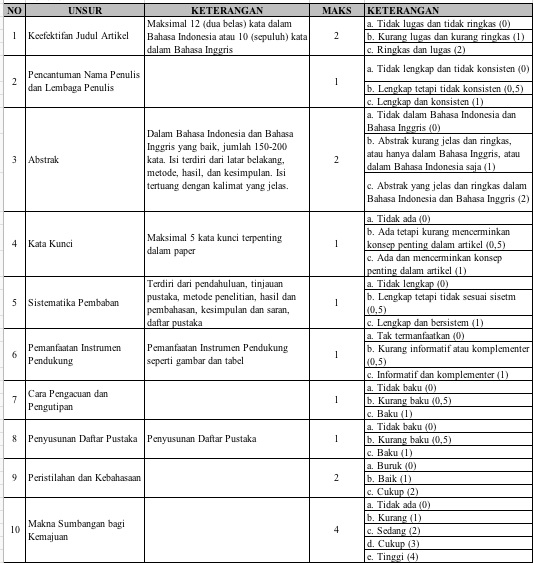
\includegraphics[width=1\textwidth]
      {figures/form1}}
      \caption{Form nilai bagian 1.}
      \label{form1}
      \end{figure}

	\begin{figure}[ht]
	      \centerline{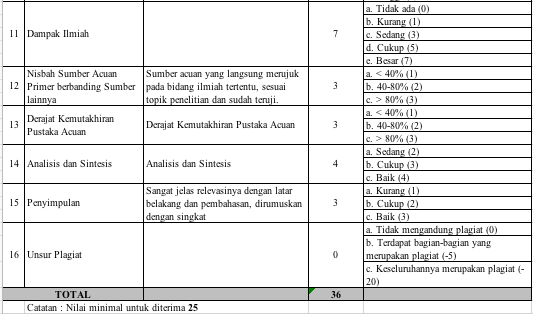
\includegraphics[width=1\textwidth]
	      {figures/form2}}
	      \caption{form nilai bagian 2.}
	      \label{form2}
	      \end{figure}

\chapter{FAQ}

M : Kalo Intership II atau TA harus buat aplikasi ?
D : Ga harus buat aplikasi tapi harus ngoding

M : Pa saya bingung mau ngapain, saya juga bingung mau presentasi apa?
D : Makanya baca de, buka jurnal topik `ganteng' nah kamu baca dulu sehari 5 kali ya, 4 hari udah 20 tuh. Bingung itu tanda kurang wawasan alias kurang baca.

M : Pa saya sudah cari jurnal terindeks scopus tapi ga nemu.
D : Kamu punya mata de? coba dicolok dulu. Kamu udah lakuin apa aja? tolong di list laporkan ke grup Tingkat Akhir. Tinggal buka google scholar klik dari tahun 2014, cek nama jurnalnya di scimagojr.com beres.

M : Pa saya belum dapat tempat intership, jadi ga tau mau presentasi apa?
D : kamu kok ga nyambung, yang dipresentasikan itu yang kamu baca bukan yang akan kamu lakukan.

M : Pa ini jurnal harus yang terindex scopus ga bisa yang lain ?
D : Index scopus menandakan artikel tersebut dalam standar semantik yang mudah dipahami dan dibaca serta bukan artikel asal jadi. Jika diluar scopus biasanya lebih sukar untuk dibaca dan dipahami karena tidak adanya proses review yang baik dan benar terhadap artikel.

M : Pa saya tidak mengerti
D : Coba lihat standar alasan

M : Pa saya bingung
D : Coba lihat standar alasan

M : Pa saya sibuk
D : Mbahmu....

M : Pa saya ganteng
D : Ndasmu....

M : Pa saya kece
D : wes karepmu lah....


Biasanya anda memiliki alasan tertentu jika menghadapi kendala saat proses bimbingan, disini saya akan melakukan standar alasan agar persepsi yang diterima sama dan tidak salah kaprah. Penggunaan kata alasan tersebut antara lain :

1. Tidak Mengerti : anda boleh menggunakan alasan ini jika anda sudah melakukan tahapan membaca dan meresumekan 15 jurnal. Sudah mencoba dan mempraktekkan teorinya dengan mencari di youtube dan google minimal 6 jam sehari selama 3 hari berturut-turut.

2. Bingung : anda boleh mengatakan alasan bingung setelah maksimal dalam berusaha menyelesaikan tugas bimbingan dari dosen(sudah dilakukan semua). Anda belum bisa mengatakan alasan bingung jika anda masih belum menyelesaikan tugas bimbingan dan poin nomor 1 diatas. Setelah anda menyelesaikan tugas bimbingan secara maksimal dan tahap 1 poin diatas, tapi anda masih tetap bingung maka anda boleh memakai alasan ini.

%next line adds the Bibliography to the contents page
\addcontentsline{toc}{chapter}{Bibliography}
%uncomment next line to change bibliography name to references
%\renewcommand{\bibname}{References}
\bibliography{references}        %use a bibtex bibliography file refs.bib
\bibliographystyle{plain}  %use the plain bibliography style

\end{document}

